\section{Localization System Evaluation}

\subsection{Experiment Setup}

The experiment is simply hanging a QR code on a wall, then calculate the user pose relative to it using the proposed localization system from different angles and distances and using different light conditions. Here more details for the setup:

\textbf{Used Cameras:}\\
This experiment will be deducted using The rear camera of Honor ALI-NX1.

\textbf{Cameras Calibration:}\\
The camera was calibrated using our implementation. It took 15 pictures of the calibration pattern at arbitrary angles and distances. We got the following re-projection errors for the camera: 0.073705403872446

This is a great value, especially that the pictures were totally random.

\textbf{QR Code Setup:}\\
The QR code will be placed on the wall(See figure \ref{Localization-Experiment-QR-Setup}) at a fixed height to simplify the measuring process.

\begin{figure}[h!]
	\centering
	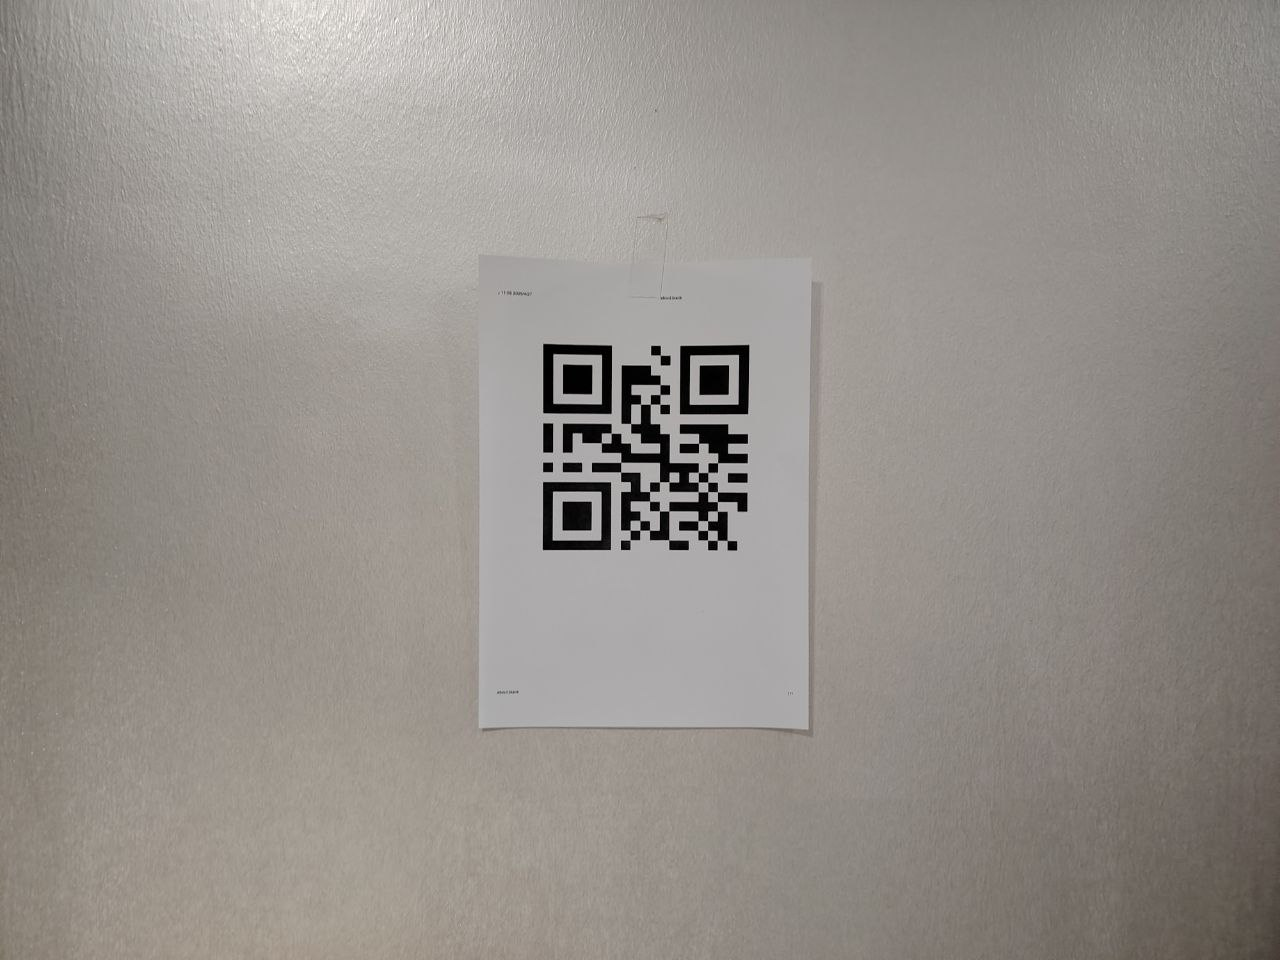
\includegraphics[width=0.7\linewidth]{assets/ch4/QR on a wall.jpg}
	\caption{A picture illustrates the QR code setup}
	\label{Localization-Experiment-QR-Setup}
\end{figure}

\textbf{Lighting Conditions:}\\
The localization performance of the camera will be tested at three distinct lighting conditions(See figure \ref{Localization-Experiment-Lighting-Conditions}):
\begin{itemize}
	\item \textbf{Perfect Lighting}
	\item \textbf{Poor Lighting}
	\item \textbf{No Lighting At All(Dark):} Here the camera's built in flash light will be used.
\end{itemize}

\begin{figure}[h!]
	\centering
	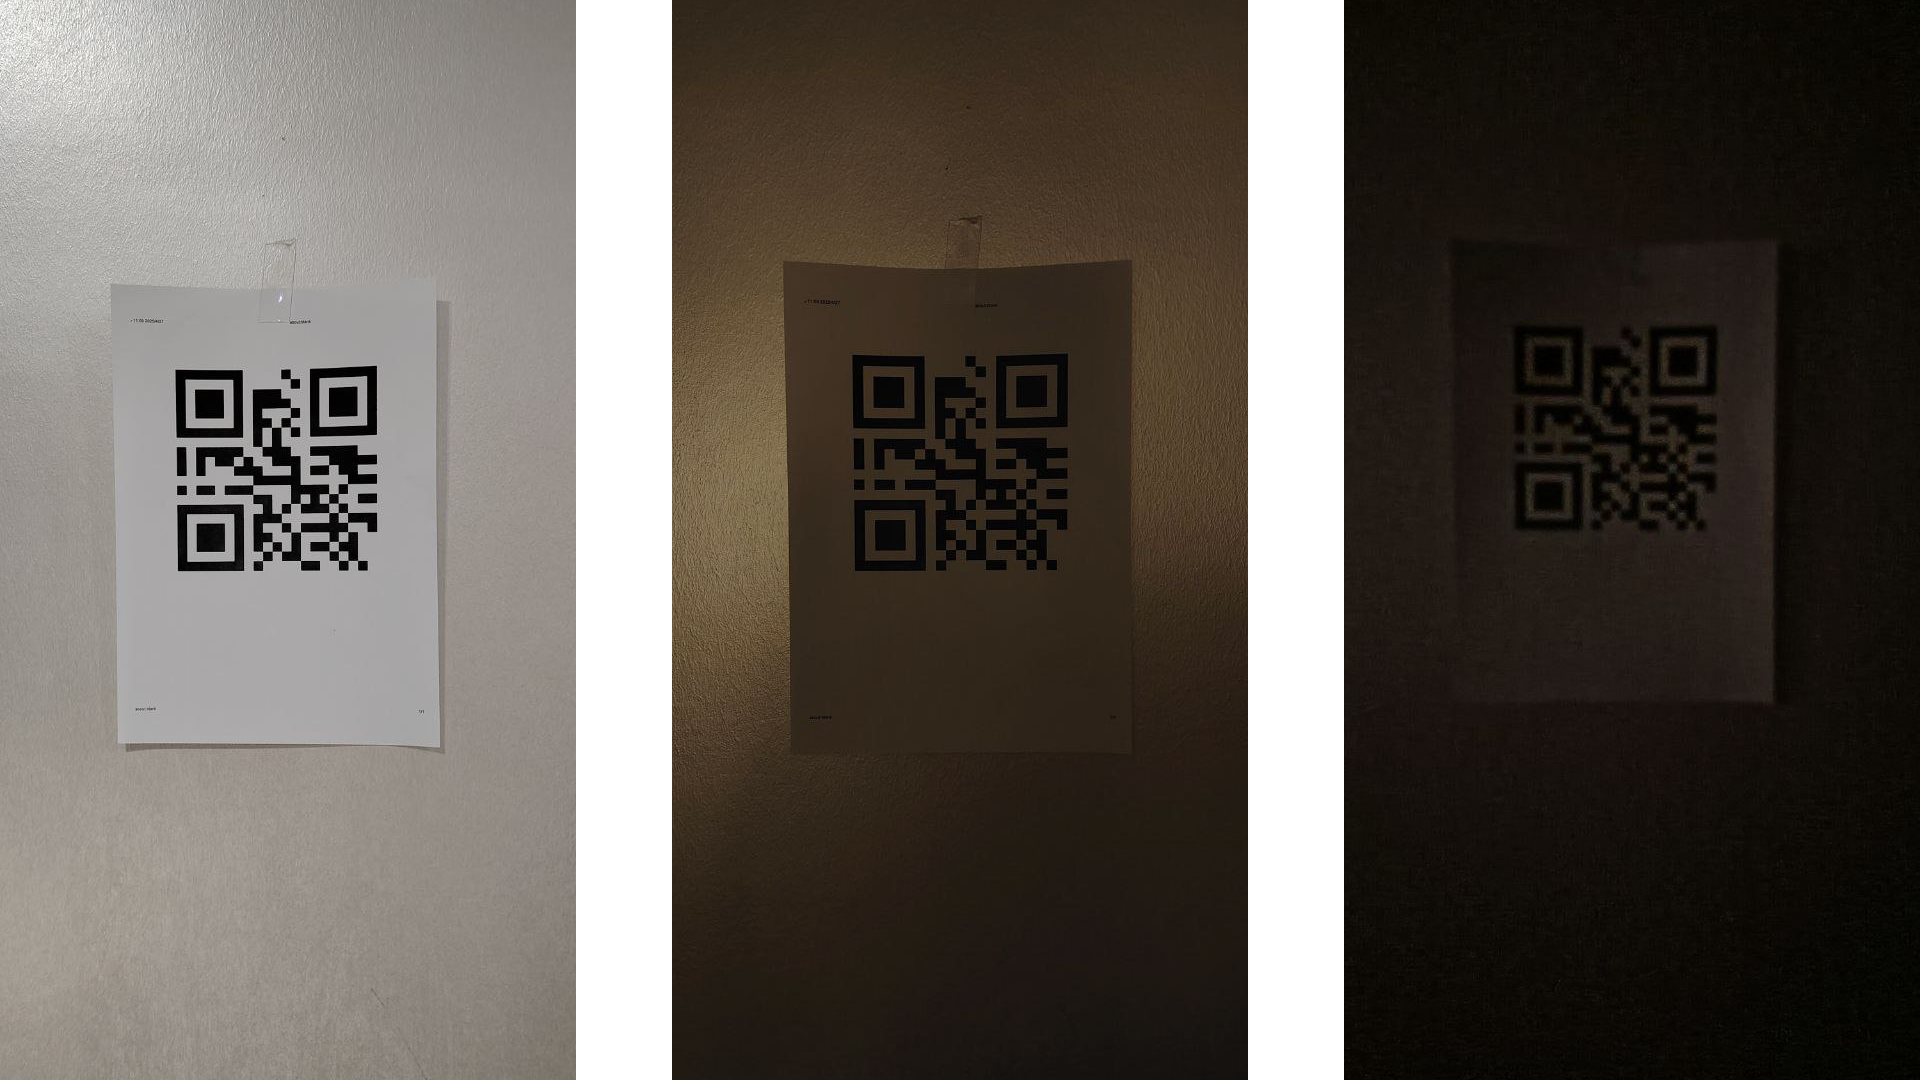
\includegraphics[width=0.7\linewidth]{assets/ch4/Three lighting conditions/Three lighting conditions.png}
	\caption{This figure illustrates the three distinct lighting conditions. The one on the left is at the perfect lighting conditions, the one on the middle is at poor lighting conditions, the one on the right is at dark.}
	\label{Localization-Experiment-Lighting-Conditions}
\end{figure}

\textbf{Measuring Tools:}
\begin{itemize}
	\item \textbf{Tape Measuring:} This will be used to measure the camera's x and y position relative to the QR code.
\end{itemize}
The measured x and y values will be used to calculate the camera's angle and distance relative to the QR code. This measuring way will give an accuracy of ±5mm, which is good enough for our application.

\subsection{Procedure}\label{sec:procedure}
The experiment will be executed three times for each lighting condition. First the localization system will be tested at a distance of 1.41 m three times for each of the following angles: 0\textdegree, +45\textdegree, and -45\textdegree. Then the same thing will be repeated for a distance of 0.707 m.

This way of testing will illustrates very well how angles, distances, and lighting conditions can or can not affect the localization performance.

\subsection{Evaluation Metrics}

The evaluation metrics applied in this experiment are described in details in Section~\ref{sec:evaluation_metrics} of the Methodology chapter. All results and analyses presented here are based on those metrics.

\subsection{Results}
The experiment results are stored in tables \ref{table:localization_exp_res_A}, \ref{table:localization_exp_res_B}, and \ref{table:localization_exp_res_C} each holding the results of the localization system estimated values with their corresponding real values for each lighting condition. The experiment results are evaluated using the metrics mentioned at Section~\ref{sec:evaluation_metrics}, and the evaluation results are stored at Table \ref{table:localization_eval}.

\begin{table}[h!]
	\caption{This tables holds the estimated values of the distances and angles with their corresponding real values in the perfect lighting condition.}
	
	\begin{tabularx}{0.8\textwidth} { 
			| >{\raggedright\arraybackslash}X 
			| >{\centering\arraybackslash}X 
			| >{\centering\arraybackslash}X 
			| >{\raggedleft\arraybackslash}X | }
		\hline
		Estimated Distance & Estimated Angle & Real Distance & Real Angle\\
		\hline
		
		0.960 m & -2.4\textdegree & 1.41 m & 0\textdegree\\
		\hline
		0.989 m & +43.2\textdegree & 1.41 m & +45\textdegree\\
		\hline
		0.981 m & -42.6\textdegree & 1.41 m & -45\textdegree\\
		\hline
		
		0.481 m & +3.1\textdegree & 0.707 m & 0\textdegree\\
		\hline
		0.496 m & +47.3\textdegree & 0.707 m & +45\textdegree\\
		\hline
		0.476 m & -42.6\textdegree & 0.707 m & -45\textdegree\\
		\hline
	\end{tabularx}
	\label{table:localization_exp_res_A}
\end{table}

\begin{table}[h!]
	\caption{This tables holds the estimated values of the distances and angles with their corresponding real values in the poor lighting condition.}
	
	\begin{tabularx}{0.8\textwidth} { 
			| >{\raggedright\arraybackslash}X 
			| >{\centering\arraybackslash}X 
			| >{\centering\arraybackslash}X 
			| >{\raggedleft\arraybackslash}X | }
		\hline
		Estimated Distance & Estimated Angle & Real Distance & Real Angle\\
		\hline
		
		0.984 m & -3.0\textdegree & 1.41 m & 0\textdegree\\
		\hline
		0.972 m & +44.5\textdegree & 1.41 m & +45\textdegree\\
		\hline
		0.946 m & -45.6\textdegree & 1.41 m & -45\textdegree\\
		\hline
		
		0.511 m & -4.3\textdegree & 0.707 m & 0\textdegree\\
		\hline
		0.485 m & +43.3\textdegree & 0.707 m & +45\textdegree\\
		\hline
		0.516 m & -47.8\textdegree & 0.707 m & -45\textdegree\\
		\hline
	\end{tabularx}
	\label{table:localization_exp_res_B}
\end{table}

\begin{table}[h!]
	\caption{This tables holds the estimated values of the distances and angles with their corresponding real values in the dark using flash light.}
	
	\begin{tabularx}{0.8\textwidth} { 
			| >{\raggedright\arraybackslash}X 
			| >{\centering\arraybackslash}X 
			| >{\centering\arraybackslash}X 
			| >{\raggedleft\arraybackslash}X | }
		\hline
		Estimated Distance & Estimated Angle & Real Distance & Real Angle\\
		\hline
		
		0.992 m & +4.2\textdegree & 1.41 m & 0\textdegree\\
		\hline
		1.014 m & +44.2\textdegree & 1.41 m & +45\textdegree\\
		\hline
		0.998 m & -44.8\textdegree & 1.41 m & -45\textdegree\\
		\hline
		
		0.501 m & +3.1\textdegree & 0.707 m & 0\textdegree\\
		\hline
		0.500 m & +42.7\textdegree & 0.707 m & +45\textdegree\\
		\hline
		0.526 m & -48\textdegree & 0.707 m & -45\textdegree\\
		\hline
	\end{tabularx}
	\label{table:localization_exp_res_C}
\end{table}

\begin{table}[h!]
	\caption{Evaluation results.}
	
	\begin{tabularx}{0.8\textwidth} { 
			| >{\raggedright\arraybackslash}X 
			| >{\centering\arraybackslash}X 
			| >{\centering\arraybackslash}X 
			| >{\centering\arraybackslash}X 
			| >{\raggedleft\arraybackslash}X | }
			
		\hline
		Lighting Condition
		&
		Distance Mean Absolute Error
		&
		Angle Mean Absolute Error
		&
		Distance Standard Deviation
		&
		Angle Standard Deviation\\
		\hline
		
		\hline
		Perfect
		&
		0.328
		&
		2.4
		&
		0.246392
		&
		35.92218
		\\
		\hline
		
		\hline
		Poor
		&
		0.323
		&
		2.15
		&
		0.232137
		&
		37.01147
		\\
		\hline
		
		\hline
		Dark
		&
		0.30333
		&
		2.2666
		&
		0.246401
		&
		36.77611
		\\
		\hline

	\end{tabularx}
	\label{table:localization_eval}
\end{table}

\subsection{Results Discussion}
As it clear from Table~\ref{table:localization_eval} the lighting conditions made no affect on the accuracy at all. Another interesting thing to notice is the fact that the angles were almost perfect unlike the distances. Actually, this is exactly what we need. Angles are needed to be close to perfection since users will be directed and a small deviation in the direction would lead to a wrong place. Meanwhile, the estimated distances will not affect the system that much. As it described at \ref{Location-Based Instructions and Information}, the system relies on both the estimated distance and the calculated distance between the current and the next milestones. For example, if the estimated distance between the user and the QR code was 2m while it is actually 2.6m, the error percentage is 23\%. But in the implementation, 2m is added to the distance between the current and the next milestones, for example 3m\footnote{In our experiments, we found that this is the average value of the distance between the current and the next milestones. Thus, we will use this value for illustration proposes assuming that it is always the average value.}, thus, the error percentage becomes 10.714\%. Table \ref{table:real_estimated_distance_error_effect} shows the real effect of the estimated distance error.

\begin{table}[h!]
	\caption{This table illustrates the actual effect of the estimated distance value errors to the system. Assuming an average milestones distance of 3m.}
	
	\begin{tabularx}{0.8\textwidth} { 
			| >{\raggedright\arraybackslash}X 
			| >{\centering\arraybackslash}X 
			| >{\centering\arraybackslash}X 
			| >{\raggedleft\arraybackslash}X | }
		\hline
		Estimated Distance & Real Distance & Fake Error Effect & Real Error Effect\\
		\hline
		0.511 m & 0.707 m & 27.722\% & 5.287\%\\
		\hline
		1.014 m & 1.41 m & 28.085\% & 8.98\%\\
		\hline
	\end{tabularx}
	\label{table:real_estimated_distance_error_effect}
\end{table}